\documentclass{beamer}
\mode<presentation>
\usepackage{amsmath}
\usepackage{amssymb}
\usepackage{mathtools}                                    
\usepackage{listings}
\usepackage{graphicx}
\usepackage{hyperref}
\usetheme{Boadilla}
\usecolortheme{lily}
\setbeamertemplate{footline}{
  \leavevmode%
  \hbox{%
    \begin{beamercolorbox}[wd=.9\paperwidth,ht=2.25ex,dp=1ex,left]{author in head/foot}%
      \hspace{1em} Arnav Makarand Yadnopavit
    \end{beamercolorbox}%
    \begin{beamercolorbox}[wd=.1\paperwidth,ht=2.25ex,dp=1ex,right]{author in head/foot}%
      \insertframenumber{} / \inserttotalframenumber\hspace*{2ex}
    \end{beamercolorbox}}%
}
\setbeamertemplate{navigation symbols}{}

\numberwithin{equation}{section}
\title{9.1.5: Solving a Differential Equation}
\author{EE24BTECH11007 - Arnav Makarand Yadnopavit}
\date{\today}

\begin{document}

\begin{frame}
\titlepage
\end{frame}

\section*{Outline}
\begin{frame}
\tableofcontents
\end{frame}

\section{Question}
\begin{frame}
\frametitle{Question}
Solve the differential equation:
\begin{align}
\frac{d^2y}{dx^2} = \cos3x + \sin3x
\end{align}
with initial conditions:
\begin{align}
y(0) = 0, \quad y^\prime(0) = \frac{1}{3}.
\end{align}
\end{frame}

\section{Solution}
\subsection{Theoretical Solution}
\begin{frame}
\frametitle{Theoretical Solution}
Integrate with respect to \(x\):
\begin{align}
    \int \frac{d^2y}{dx^2} dx &= \int \cos3x + \sin3x \, dx, \\
    \frac{dy}{dx} &= \frac{\sin3x}{3} - \frac{\cos3x}{3} + c_1.
\end{align}
Using \(y^\prime(0) = \frac{1}{3}\):
\begin{align}
c_1 = 0.
\end{align}
Integrate again:
\begin{align}
y = -\frac{\cos3x}{9} - \frac{\sin3x}{9} + c_2.
\end{align}
Using $y(0) = 0$:
\begin{align}
c_2 = \frac{1}{9}.
\end{align}
\begin{align}
\therefore y = -\frac{\cos3x}{9} - \frac{\sin3x}{9} + \frac{1}{9}.
\end{align}
\end{frame}

\subsection{Computational Solution}
\begin{frame}
\frametitle{Computational Solution}
\begin{align}
y^\prime(x) = \frac{\sin3x}{3} - \frac{\cos3x}{3}.
\end{align}
Let the Laplace transform of RHS be \(X(s)\). Then,
\begin{align}
g(t) = \frac{\sin3t}{3} - \frac{\cos3t}{3}.
\end{align}
\begin{align}
\frac{dy}{dt} = g(t).
\end{align}
Applying Laplace transform on both sides, we have
\begin{align}
s Y(s) = X(s)
\end{align}
The transfer function, $H(s)$ can then be defined as
\begin{align}
	H(s) &= \frac{Y(s)}{X(s)} \\
	H(s) &= \frac{1}{s} \label{eq:bil}
\end{align}
\end{frame}
\begin{frame}{Computational Solution}
Applying \textbf{Bi-linear transform} on both sides of \eqref{eq:bil}, i.e., converting \(s\)-domain into \(z\)-domain, we have:
\begin{align}
    s &= \frac{2}{h} \frac{1 - z^{-1}}{1 + z^{-1}}, \\
    ROC&: |z|>1\\
    H(z) &= \frac{h}{2} \frac{1 + z^{-1}}{1 - z^{-1}}, \\
    Y(z) &= \frac{h}{2} \frac{1 + z^{-1}}{1 - z^{-1}} X(z), \\
    (1 - z^{-1}) Y(z) &= \frac{h}{2} \left(1 + z^{-1}\right) X(z). \label{eq:iz}
\end{align}
The resulting difference equation becomes:
\begin{align}
    y_{n} = y_{n-1} + \frac{h}{2} \left[ g(x_n) + g(x_{n-1}) \right].
\end{align}
\end{frame}


\subsection{Graphical Representation}
\begin{frame}
\frametitle{Graphical Representation}
\begin{figure}[h]
    \centering
    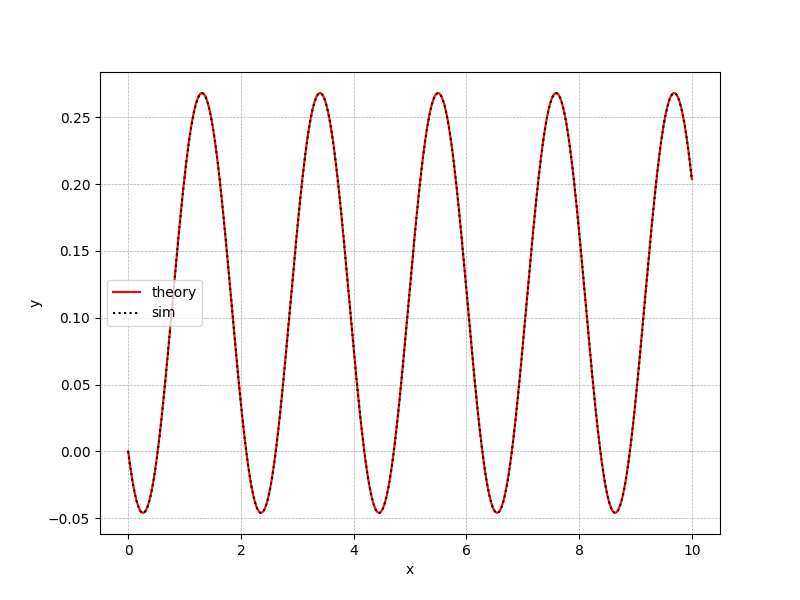
\includegraphics[width=\columnwidth]{figs/fig.png}
    \caption{Graphical solution of the differential equation.}
\end{figure}
\end{frame}

\end{document}

